{
    \subsubsection{Տվյալների բազայի նախագծում}\label{subsubsec:database}

    Հարցումները արդյունավետ կատարելու նպատակով նախագծվել է տվյալների բազա՝ հաշվի առնելով ռելացիոն ու ոչ ռելացիոն
    բազաների հատկությունները։ Տվյալների բազան ներառում է աղբյուր կոդի հիմնական տարրերի՝ դասերի, դասերի անդամ դաշտերի
    և հրահանգների մասին տեղեկություններ (Նկար \ref{fig:figure7}):

    \begin{figure}[h]
        \centering
        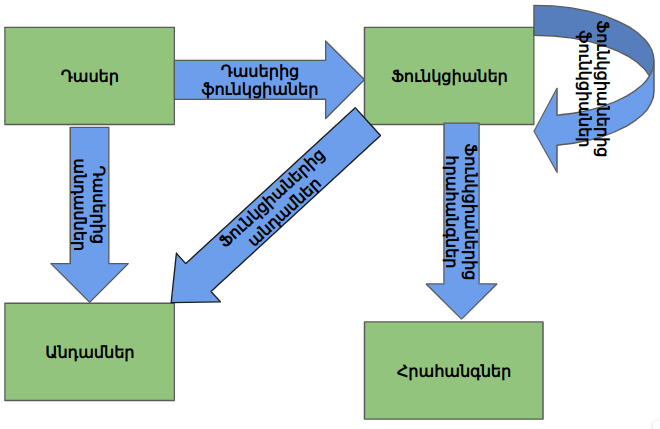
\includegraphics[width=0.8\textwidth]{pic7}
        \caption{Տվյալների բազայի կառուցվածքը}
        \label{fig:figure7}
    \end{figure}
}